\documentclass[10pt]{beamer}
\usetheme{metropolis}  
\usecolortheme{dove}
\usepackage{hyperref}
\usepackage{bigints}
\usepackage{amsmath}
\title{Introducci\'on a la probabilidad y estad\'istica CM274}
 \usepackage[spanish]{babel}
 \decimalpoint
\date{\today}
\author{C\'esar Lara Avila}
\institute{\url{https://github.com/C-Lara}}
\begin{document}
  \maketitle
  \section{5. Esperanza de variables aleatorias discretas }
  
\begin{frame}{Ejemplos iniciales}
\small {\textbf{Ejemplo 1:} Supongamos que tenemos un dado de seis lados marcado con cinco  $3$ y un $6$. ?`Cu\'al seria  el promedio de $6000$ lanzamiento?
	
Si supi\'eramos el valor de cada lanzamiento, podr\'iamos calcular el promedio sumando los $6000$ valores y dividi\'endolos por $6000$. Sin conocer los valores, podemos calcular el promedio esperado como sigue.

Dado que hay cinco $3$ y un $6$ esperamos que aproximadamente $5/6$ de los lanzamientos dar\'a $3$ y $1/6$ dar\'a $6$. Suponiendo que esto sea exactamente cierto, tenemos la siguiente tabla de valores y conteos

\begin{table}[]
	\centering
	\begin{tabular}{ccc}
		valores:        & 3    & 6    \\
		conteo esperado: & 5000 & 1000
	\end{tabular}
\end{table}

El promedio de esos $6000$ valores es entonces

\[
\frac{5000\cdot 3 + 1000\cdot 6}{6000} = \frac{5}{6}\cdot 3 + \frac{1}{6}\cdot 6 = 3.5
\]


}
\end{frame}

\begin{frame}{Ejemplos iniciales (continuaci\'on)}
\small{Consideramos que este es el promedio esperado en el sentido de que \texttt{esperamos} que cada uno de los valores posibles ocurra con las frecuencias dadas.

\textbf{Ejemplo 2:} Lanzamos dos dados est\'andar de $6$ caras. Ganamos $S/. 1000$ si la suma es $2$ y pierde $S/.100$ en caso contrario. ?`Cu\'anto se espera ganar en promedio por lanzamiento?.

La probabilidad de un $2$ es $1/36$. Si tu juegas $N$ veces, puedes \texttt{esperar} $\frac{1}{36}\cdot N$ de los lanzamientos da un $2$ y $\frac{35}{36}\cdot N$ de los lanzamientos puede dar algo m\'as. As\'i sus ganancias  totales esperadas

\[
1000\cdot \frac{N}{36} - 100\cdot \frac{35N}{36}.
\]	

Para obtener el promedio esperado por lanzamiento, dividimos el total por $N$:

\[
\text{promedio esperado} = 1000\cdot \frac{1}{36} - 100\cdot \frac{5}{36} = -69.44.
\]
}


\end{frame}

\begin{frame}{Definici\'on de esperanza}
\small{Se debe  observar que en ambos ejemplos la suma para el promedio esperado consta de t\'erminos que son un valor de la variable aleatoria multiplicada por su probabilidad. Esto lleva a la siguiente definici\'on.
	
Supongamos que $X$ es una variable aleatoria discreta que toma valores $x_1, x_2,\dots, x_n$ con probabilidades $p(x_1), p(x_2), \dots, p(x_n)$. La esperanza o valor esperado de $X$ es denotado por $\mathbb{E}(X)$ y definida como}

\[
\mathbb{E}{(X)} = \sum_{j =1}^{n}p(x_j)x_j = p(x_1)x_1 + p(x_2)x_2 + \dots p(x_n)x_n.
\]	
	
\textbf{Notas}

\begin{itemize}
	\scriptsize{
	\item El valor esperado tambi\'en se denomina \textcolor{orange}{media} o \textcolor{blue}{promedio} de $X$ y a menudo se indica por $\mu$.
	\item La esperanza  proporciona una medida de la localizaci\'on de la tendencia central de una variable aleatoria.
	\item Si todos los valores son igualmente probables entonces el valor esperado es s\'olo el promedio habitual de los valores.
}
\end{itemize}
	
\end{frame}

\begin{frame}{Ejemplos }
\scriptsize{ \textbf{Ejemplo 3:} Sea $X$ una variable aleatoria $\text{Bernoulli}(p)$. Como $X$ toma los valores $0$ y $1$, con probabilidades $p$ y $1 -p$, la esperanza se calcula como

\[
\mathbb{E}(X) = p\cdot 1 + (1 -p)\cdot 0 = p. 
\]	

\textbf{Ejemplo 4:} Sea $X$ una variable aleatoria $\text{Binomial}(n, p)$. Por definici\'on, la media de la distribuci\'on binomial es dada por

\begin{align*}
\mu &= \mathbb{E}(X) = \sum_{k = 0}^{n}kp(k) = \sum_{k =1}^{n}k\frac{n!}{k!(n -k)!}p^kq^{n -k} \\
 &= np\sum_{k =1}^{n}\frac{(n -1)!}{(k -1)!(n -k)!}p^{k -1}q^{n -k} = np\sum_{x =0}^{n -1}\binom{n -1}{x}p^xq^{n -1 -x}\\
 &= np(p +q)^{n -1} = np.\\
\end{align*}


\textbf{Ejemplo 5:} Sea $X$ una variable aleatoria $\text{Geometrica}( p)$. Calculemos $\mathbb{E}(X)$. De manera usual, la esperanza de la distribuci\'on geom\'etrica es  (donde  $q = 1 -p$)

\begin{align*}
\mathbb{E}(X) &= \sum_{k =0}^{\infty}kq^{k}p = pq\sum_{k =0}^{\infty}kq^{k -1} = pq\frac{1}{(1 -q)^2} = \frac{q}{p}.
\end{align*}
}
\end{frame}

\begin{frame}{Media y centro o masa}
\small{Podriamos habernos preguntado por que usamos el nombre de  \textcolor{red}{funci\'on de masa de probabilidad}. Esta es la raz\'on: si colocamos un objeto de masa $p(x_j)$ en la posici\'on $x_j$ para cada $j$, entonces $\mathbb{E}(X)$ es la posici\'on del centro de masa. Recordemos esta \'ultima noci\'on a trav\'es de un ejemplo.
	
\textbf{Ejemplo 6:} Supongamos que tenemos dos masas a lo largo del eje $x$, la masa $m_1 = 500$ en la posici\'on $x_1 = 3$ y la  masa $m_2 = 100$ en la posici\'on $x _2 = 6$. ?`D\'onde se encuentra el centro de masa?.
	
Intuitivamente sabemos que el centro de masa est\'a m\'as cerca de la masa mayor.

\begin{figure}[ht]
	\centering
	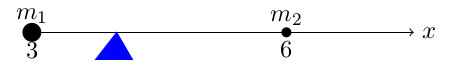
\includegraphics[width=6cm]{g1}
\end{figure}

	}
\end{frame}

\begin{frame}{Continuaci\'on \dots }
\small{ De la f\'isica sabemos que el centro de masa es
		
\[
\overline{x} = \frac{m_1x_1 + m_2x_2}{m_1 + m_2} = \frac{500\cdot 3 + 100\cdot 6 }{600} = 3.5
\]

\vspace{0.2cm}

Llamamos a esta f\'ormula un promedio ponderado de $x_1$ y $x_2$. Aqu\'i $x_1$ se pesa m\'as fuertemente porque tiene m\'as masa.

\vspace{0.2cm}

Ahora veamos la definici\'on de valor esperado $\mathbb{E}(X)$. Es una media ponderada de los valores de $X$ siendo los pesos las probabilidades $p(x_i)$ en lugar de las masas!. Podr\'iamos decir que \texttt{el valor esperado es el punto en el que la distribuci\'on se equilibrar\'ia}.	
	}
	
\end{frame}


\begin{frame}{Propiedades algebraicas de $\mathbb{E}(X)$}
\small{El valor esperado $\mathbb{E}(X)$ de variables aleatorias  es lineal.
	
\begin{enumerate}
	\item Si $X$ e $Y$ son variables aleatorias de un espacio muestral $\Omega$, entonces
	
	\[
	\mathbb{E}(X + Y) = \mathbb{E}(X) + \mathbb{E}(Y).
	\]
\item Si $a$ y $b$ son constantes, entonces

\[
\mathbb{E}(aX + b) = a\mathbb{E}(X) + b.
\]
\end{enumerate}	


\vspace{0.3cm}

\scriptsize{
	
\textbf{Ejemplo 7:} Lanzamos dos dados y $X$ sea la suma, sea $X_1$ el valor en el primer dado y $X_2$ sea el valor del segundo dado. Como $X = X_1 + X_2$ tenemos $\mathbb{E}(X) = \mathbb{E}(X_1) + \mathbb{E}(X_2)$. Se calcula que $\mathbb{E}(X_1) = \mathbb{E}(X_2) = 3.5$, por lo tanto $\mathbb{E}(X) = 7$.

\textbf{Ejemplo 8:} (Para las variables aleatorias infinitas la media no siempre existe.) Supongamos que $X$ tiene un n\'umero infinito de valores seg\'un la siguiente tabla

\begin{table}[]
	\centering
	\begin{tabular}{ccccccc}
		valores $x$   & $2$   & $2^2$   & $2^3$   & \dots   & $2^k$   & \dots   \\
		PMF $p(x)$ & $1/2$ & $1/2^2$ & $1/2^3$ & \dots & $1/2^k$ & \dots
	\end{tabular}
\end{table}

Calculemos la media : $\displaystyle \mathbb{E}(X) = \sum_{k =1}^{\infty}2^k\frac{1}{2^k} = \sum_{k =1}^{\infty}1 = \infty.$
}
	
}

\end{frame}


\begin{frame}{Pruebas de las propiedades algebr\'aicas de $\mathbb{E}(X)$}
\small{ La prueba de la propiedad (1) es simple, pero hay alguna sutileza en la comprensi\'on de lo que significa a\~nadir dos variables aleatorias. Recordemos que el valor de la variable aleatoria es un n\'umero determinado por el resultado de un experimento. Agregar $X$ e $Y$ significa agregar los valores de $X$ e $Y$ para el mismo resultado. En forma de tabla esto se parece a:
	
\begin{table}[]
	\centering
	\begin{tabular}{llllll}
		salida $\omega$           & $\omega_1$             & $\omega_2$             & $\omega_3$             & \dots & $\omega_n$             \\
		valores de $X$            & $x_1$                  & $x_2$                  & $x_3$                  & \dots & $x_n$                  \\
		valores de $Y$            & $y_1$                  & $y_1$                  & $y_3$                  & \dots & $y_n$                  \\
		valores de $X +Y$         & $x_1 + y_1$            & $x_2 + y_2$            & $x_3 + y_3$            & \dots & $x_n + y_n$            \\
		prob $\mathbb{P}(\omega)$ & $\mathbb{P}(\omega_1)$ & $\mathbb{P}(\omega_2)$ & $\mathbb{P}(\omega_3)$ & \dots & $\mathbb{P}(\omega_n)$
	\end{tabular}
\end{table}	

La prueba de (1) se sigue inmediatamente:

\[
\mathbb{E}(X + Y) = \sum(x_i + y_i)\mathbb{P}(\omega_i) = \sum x_i\mathbb{P}(\omega_i) + \sum y_i\mathbb{P}(\omega_i) = \mathbb{E}(X) + \mathbb{E}(Y).
\]
}
\end{frame}

\begin{frame}{continuaci\'on \dots}
\small{

La prueba de la propiedad (2) toma una l\'inea.

\[
\mathbb{E}(aX + b) = \sum p(x_i)(ax_i + b) = a\sum p(x_i)x_i + b\sum p(x_i) = a\mathbb{E}(X) + b.
\]

El t\'ermino $b$ en la \'ultima expresi\'on se debe a que $\displaystyle \sum p(x_i) =1$.}

\vspace{0.8 cm}

\scriptsize{
\textbf{Ejemplo 9:} Michael Jordan, el mejor jugador de baloncesto de todos los tiempos, hizo el $80\%$ de sus tiros libres. En un juego cu\'al es el n\'umero esperado que har\'ia antes de su primera falta.

Aqu\'i hay un ejemplo donde queremos el n\'umero de \'exitos antes de la primer fracaso. Usando el lenguaje neutral de caras y colas: el \'exito es sello (probabilidad $1 - p$) y el fracaso es cara (probabilidad = $p$). Por lo tanto $p =.2$ y el n\'umero de sellos (lanzamientos libres) antes de la primera cara (tiro libre p\'erdido) es modelado por un $X \sim \text{Geometrica(.2)}$. Luego por el Ejemplo 5, tenemos, 

\[
\mathbb{E}(X) = \frac{1 - p}{p}= \frac{.8}{.2} = 4.
\]

}

\end{frame}

\begin{frame}{Variable aleatoria indicador}
\small{ La variable aleatoria indicador $I_A$ (o $I(A)$) para un evento $A$ se define como $1$ si $A$ ocurre y $0$ en caso contrario. As\'i  $A$ es una variable aleatoria de Bernoulli, donde el \'exito se define como \texttt{$A$ ocurre} y el fracaso se define como \texttt{$A$ no ocurre}.
	
Algunas propiedades \'utiles del indicador  se resumen a continuaci\'on.

\begin{itemize}
	\item $(I_A)^k = I_A$ para alg\'un entero $k$.
	\item $I_{A^c} = 1 -I_A$.
	\item $I_{A \cap B} = I_AI_B$.
	\item $I_{A \cup B} = I_A + I_B - I_AI_B$.
\end{itemize}
	
Hay una correspondencia uno a uno entre los eventos y la variable aleatoria indicador  y la probabilidad de un evento A es el valor esperado de su variable aleatoria  indicador $I_A$ :

\begin{equation}
\mathbb{P}(A) = \mathbb{E}(I_A).
\end{equation}
}
\end{frame}


\begin{frame}{Un problema del Putnam}
	
\scriptsize{ Sea $S = \{1, 2, \dots, n\}$ para alg\'un entero $n > 1$. Decimos que una permutaci\'on $\pi$ de $S$ tiene un m\'aximo local en $j \in S$ si
	
\begin{itemize}
	\item $\pi(j) > \pi(j + 1)$ para $j =1$;
	\item $\pi(j -1) < \pi(j)$ y $\pi(j) > \pi(j + 1)$ para $1 < j < n$;
	\item $\pi(j -1) < \pi(j)$ para $j = n$.
\end{itemize}

Por ejemplo si $n = 5$ y $\pi$ toma valores en $1, 2, 3, 4, 5$ de $2, 1, 4, 5, 3$, entonces $\pi$ tiene un m\'aximo local de $2$ en $k =1$ y un m\'aximo local de $5$ en $k =4$. Para $n \geq 2$, ?`cu\'al es el n\'umero promedio de m\'aximos locales de una permutaci\'on aleatoria de $1, 2,\dots, n$, con todos las $n!$ permutaciones igualmente probables?
}

\scriptsize{ Sea $I_1 , \dots, I_n$} las variables aleatorias indicadoras, donde $I_j$ es $1$ si hay un m\'aximo local en la posici\'on $j$ y $0$ en otros casos. Estamos interesados en la esperanza de $\displaystyle \sum_{j =1}^{n}I_j$.

Para $1 < j < n, \mathbb{E}(I_j) = 1/3$, desde que tener un m\'aximo local en $j$ es equivalente a $a_j$ siendo el mayor de $a_{j -1}, a_j, a_{j +1}$, que tiene probabilidad $1/3$, desde que todos los \'ordenes son igualmente probables. Para $j =1$ o $j =n$, tenemos $\mathbb{E}(I_j) = 1/2$, desde que hay solo un vecino. As\'i por linealidad,

\[
\mathbb{E}\biggl(\sum_{j =1}^{n}I_j \biggr) = 2\cdot\frac{1}{2} + (n -2)\cdot\frac{1}{3} = \frac{n + 1}{3}.
\]

\end{frame}
\begin{frame}{Esperanza de funciones de una variable aleatoria}
\small{ Si $X$ es una variable aleatoria discreta, tomando los valores $x_1, x_2, \dots$ y $h$ es una funci\'on, $h(X)$ es una nueva variable aleatoria. La esperanza o valor esperado es

\[
\mathbb{E}(h(X)) = \sum_{j}h(x_j)p(x_j).
\]	

\textbf{Ejemplo 10: } Sea $X$ el valor de un lanzamiento de un dado y sea $Y = X^2$. Encuentra $E(Y)$.

Desde que hay un n\'umero peque\~no de valores, podemos hacer una tabla.

\begin{table}[]
	\centering
	\begin{tabular}{ccccccc}
		X    & 1   & 2   & 3   & 4   & 5   & 6   \\
		Y    & 1   & 4   & 9   & 16  & 25  & 36  \\
		prob & 1/6 & 1/6 & 1/6 & 1/6 & 1/6 & 1/6
	\end{tabular}
\end{table}


}
\end{frame}

\begin{frame}{Esperanza de funciones de una variable aleatoria (1)}

\small{Observe que la probabilidad para cada valor de $Y$ es la mismo que el  valor de $X$ correspondiente. Asi que,

\[
\mathbb{E}(Y) = \mathbb{E}{(X^2)} = 1^2\cdot \frac{1}{6} + 2^2\cdot\frac{1}{6} + \dots + 6^2\cdot \frac{1}{6} = 15.167.
\]

\vspace{0.2cm}

 \textbf{Ejemplo 11: } Lanzamos dos dados y sea $X$ su suma. Supongamos que la función de pago est\'a dada por $Y = X^2 - 6X + 1$. ?`Es una buena apuesta?.}
	
\scriptsize{En efecto $\mathbb{E}(Y) = \displaystyle\sum_{j =2}^{12}(j^2 -6j + 1)p(j)$, donde $p(j) = \mathbb{P}(X= j)$.

\begin{table}[]
	\centering
	\begin{tabular}{cccccccccccc}
		X    & 2    & 3    & 4    & 5    & 6    & 7    & 8    & 9    & 10   & 11   & 12   \\
		Y    & -7   & -8   & -7   & -4   & 1    & 8    & 17   & 28   & 41   & 56   & 73   \\
		prob & 1/36 & 2/36 & 3/36 & 4/36 & 5/36 & 6/36 & 5/36 & 4/36 & 3/36 & 2/36 & 1/36
	\end{tabular}
\end{table}

Aqu\'i el valor es $\mathbb{E}(Y) = 13.833$.  Para responder a la pregunta anterior: ya que la ganancia esperada es positiva, parece una apuesta que vale la pena tomar.	
}

\small{\textbf{Pregunta:}} Si $Y = h(X)$ hace que $\mathbb{E}(Y) = h(\mathbb{E}(X))$?.
\end{frame}

\begin{frame}{Esperanza de funciones de una variable aleatoria (2)}
\small{Dado una variable aleatoria discreta $X$ con un conjunto posible de valores $A$ y la funci\'on de masa de probabilidad $p_X(x)$, la esperanza de un nueva variable aleatoria $Y$, que es una funci\'on de $X$, es decir  $Y = h(X)$ se puede escribir como
	

\begin{equation*}
\mathbb{E}(Y) = \mathbb{E}(h(X)) = \sum_{x \in A}h(x)p_X(x).
\end{equation*}
	
	\vspace{0.2cm}
	
En efecto, sea $\Omega$ un espacio muestral. Sea $h :\mathbb{R} \rightarrow \mathbb{R}$, una funci\'on de variable real y $X: \Omega \rightarrow A \subseteq \mathbb{R}$ es una variable aleatoria con el conjunto de posibles de valores $A$. Como se sabe, $h(X)$, la composici\'on de $g$ y $X$ es una funci\'on desde $\Omega$ al conjunto $h(A) = \{h(x): x\in A\}$. As\'i $h(X)$ es una variable aleatoria con un posible conjunto de valores $g(A)$. Ahora por definici\'on de esperanza
	
	\vspace{0.2cm}

\[
\mathbb{E}(h(X)) = \sum_{z \in h(A)}z\mathbb{P}(h(X) = z)
	\]
	
}

\end{frame}

\begin{frame}{Un resultado}
\small{ Sea $X$ una variable aleatoria no negativa entera. Sea $F$ el $CDF$ de $X$ y $G(x) = 1 -F(x) = \mathbb{P}(X > x)$. La funci\'on $G$ es llamada \textcolor{red}{funci\'on de supervivencia} de $X$. Entonces
	
\[
\mathbb{E}(X) = \sum_{n = 0}^{\infty}G(n).
\]	

En efecto, para el caso en $X$ es acotada (existe un n\'umero entero no negativo $b$ , tal que $X$ es siempre como m\'aximo $b$), podemos representar como la suma de variables aleatorias indicadoras, $X = I_1 + I_2 + \cdots + I_b$, donde  $I_n = I(X \geq n)$.


Entonces se tiene, por linealidad, la ecuaci\'on (1) y el hecho que $\{ X \geq k\}$ es el mismo evento que $\{ X > k-1\}$.

\[
\mathbb{E}(X) = \sum_{k =1}^{b}\mathbb{E}(I_k) = \sum_{k =1}^{b}\mathbb{P}(X \geq k) = \sum_{n = 0}^{b -1}\mathbb{P}(X > n) = \sum_{n = 0}^{\infty}G(n).
\]
}
\end{frame}
\end{document}